\documentclass{beamer}
\usecolortheme{beaver}

% Fonts
\usepackage{fontspec}
\setmainfont{Source Serif Pro}[Ligatures=TeX]
\setsansfont{Source Sans Pro}[Ligatures=TeX]
\setmonofont{Source Code Pro}[
  BoldFont={* Medium},
  BoldItalicFont={* Medium Italic},
]

\usepackage{minted}
\usepackage{tikz}
\usetikzlibrary{positioning}

\tikzset{
  invisible/.style={opacity=0,text opacity=0},
  highlight/.style={color=red},
  intro/.code args={<#1>}{%
    \only<#1>{\pgfkeysalso{highlight}}
    \alt<#1->{}{\pgfkeysalso{invisible}}
  },
}

\title{MIRterpreter}
\subtitle{
  An interpreter for the Rust compiler's mid-level intermediate representation}
\author{Scott Olson}

\begin{document}

\maketitle

\begin{frame}
  \frametitle{Rust compilation passes}

  \begin{center}
    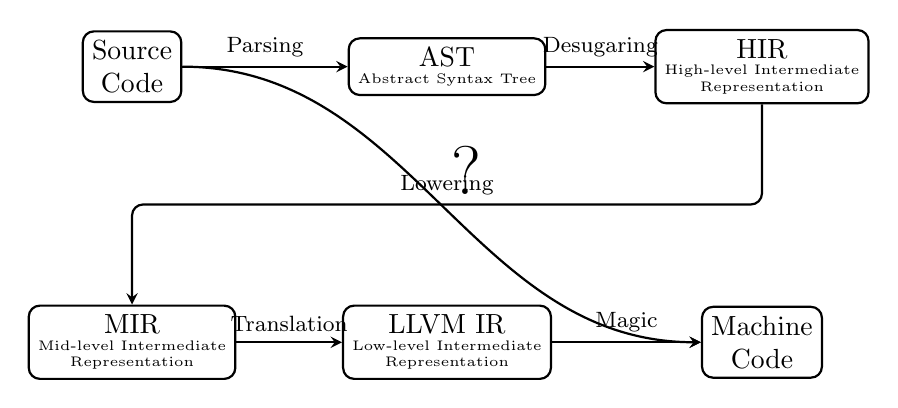
\begin{tikzpicture}[x=4cm, y=3.5cm, auto, rounded corners]
      \tikzstyle{basic-stage}=[rectangle, draw, thick, align=center]
      \tikzstyle{stage}=[basic-stage, font=\tiny]
      \tikzstyle{pass}=[thick, -stealth]
      \tikzstyle{pass-label}=[font=\footnotesize]

      \node[basic-stage] (src) at (0,0) {Source\\Code};
      \node[basic-stage] (mach) at (2,-1) {Machine\\Code};

      \draw<1>[pass, out=0, in=180]
        (src.east) to node[font=\Huge] {?} (mach.west);

      \node[stage, intro=<2>] (ast) at (1,0)
        {\normalsize{AST} \\ Abstract Syntax Tree};
      \draw[pass, intro=<2>]
        (src) -- node[pass-label] {Parsing} (ast);

      \node[stage, intro=<3>] (hir) at (2,0)
        {\normalsize{HIR} \\ High-level Intermediate\\Representation};
      \draw[pass, intro=<3>]
        (ast) -- node[pass-label] {Desugaring} (hir);

      \node[stage, intro=<4>] (mir) at (0,-1)
        {\normalsize{MIR} \\ Mid-level Intermediate\\Representation};
      \path (hir.south) -- coordinate (middle) (mir.north);
      \draw[pass, intro=<4>]
        (hir.south) |- (middle) -| (mir.north);
      \node[pass-label, above, intro=<4>] at (middle) {Lowering};

      \node[stage, intro=<5>] (llvm) at (1,-1)
        {\normalsize{LLVM IR} \\ Low-level Intermediate\\Representation};
      \draw[pass, intro=<5>]
        (mir) -- node[pass-label] {Translation} (llvm);

      \draw<6->[pass, intro=<6>]
        (llvm) -- node[pass-label] {Magic} (mach);
    \end{tikzpicture}
  \end{center}
\end{frame}

\begin{frame}[fragile]
  \frametitle{Example Rust code}
  \inputminted{rust}{code.rs}
\end{frame}

\begin{frame}[fragile]
  \frametitle{OMG TEXT}

  \begin{itemize}
    \item This is some plain old basic text. It keeps going for a while, maybe
      even long enough to wrap to the next line. No, almost surely. There it
      goes. It did it. Consider this line wrapped.

    \item This is the next bit of text.

    % \item What if I told you I had an \mintinline{rust}{impl} for a
    %   \mintinline{rust}{trait Foo}?
  \end{itemize}
\end{frame}

\end{document}
